
%%%%%%%%%%%%%%%%%%%%%%%%%%%%%%%%%%%%%%%%%%%%%%%%%%%%%%%%%%%%%%%%%%%%%%%
\subsection{Was kann überwacht werden}
%%%%%%%%%%%%%%%%%%%%%%%%%%%%%%%%%%%%%%%%%%%%%%%%%%%%%%%%%%%%%%%%%%%%%%%
\begin{frame}
\frametitle{Aktive Überwachung}
\framesubtitle{Was kann überwacht werden?}
    \pause
    \begin{alertblock}{}
        \centering{Jede Entität, deren Status deutlich zueinander abgrenzbar sind.}
    \end{alertblock}

    \vspace{0.5cm}

    \begin{columns}
        \pause
        \column{0.48\textwidth}
            \begin{itemize}
                \item Betriebssystem\color{red}abhängig
                    \begin{itemize}
                        \item Betriebssystemparameter
                        \begin{itemize}
                            \item   Auslastung
                            \item   Speicher
                            \item   Prozesse
                            \item   Datendurchsatz
                        \end{itemize}
                        \item Updates
                        \item Sicherheitsauditierung
                    \end{itemize}
             \end{itemize}
        \pause
        \column{0.48\textwidth}
        \begin{itemize}
            \item Betriebssystem\color{red}unabhängig
            \begin{itemize}
                \item Netzwerkdienste
                \begin{itemize}
                    \item L3:   ICMP\{4,6\}
                    \item L4:   TCP, UDP - basierend
                    \item L4+:  SNMP
                \end{itemize}
                \item Sensoren
                \item Aktive Netzwerkkomponenten
            \end{itemize}
        \end{itemize} 
    \end{columns}




\end{frame}

\begin{frame}
\frametitle{Visualisierungen}
\framesubtitle{Statusverlauf}

    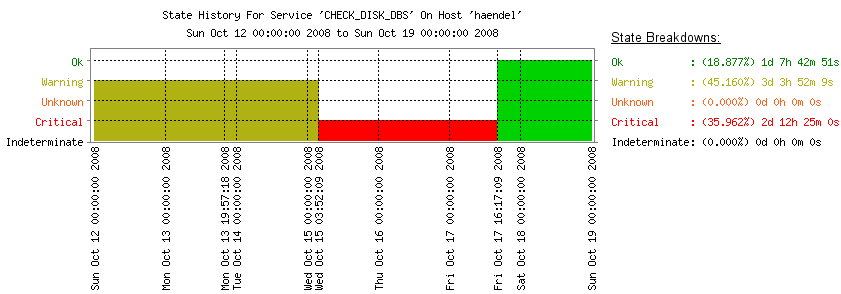
\includegraphics[scale=0.45]{img/nag_trend.png}
    \vspace{0.5cm}
    
    \footnoterule
    \footnotesize{
        Quelle:          selbst erstellt\\
        Erstellt mit:    NagVis}

\end{frame}
\begin{frame}
\frametitle{Visualisierungen}
\framesubtitle{packets/time}

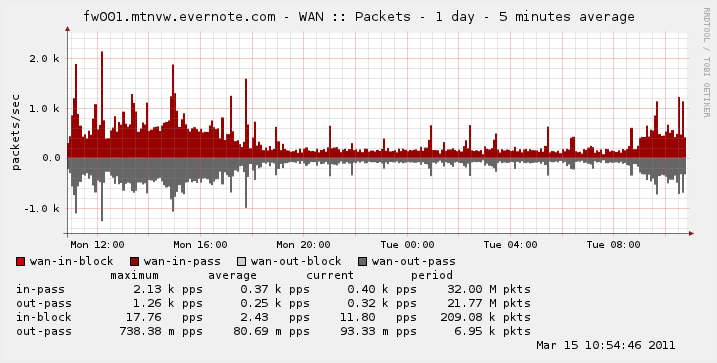
\includegraphics[scale=0.4]{img/status_rrd_graph_img.png}
\vspace{0.5cm}

\footnoterule
\footnotesize{
   Quelle:          https://redmine.pfsense.org/issues/1354\\
   Erstellt mit:    https://oss.oetiker.ch/rrdtool/}


\end{frame}